\documentclass[11pt]{article}
\usepackage[letterpaper,textwidth=5.5in,top=1in,bottom=1in]{geometry}
\usepackage{amsmath,amssymb}
\usepackage{graphicx}
\usepackage{booktabs}
\usepackage{multirow}
\usepackage{natbib}
\usepackage{microtype}
\usepackage{xurl}
\usepackage[hidelinks]{hyperref}


\title{Investigating the Impact of Losses on FGVC Performance and Geometry\\[2pt]
\large Loss-function ablation and species-count scaling ladder on SWIN-Base\\[2pt]
\normalsize Internal draft: results so far}
\author{Farid Karimli}
\date{\today}

\setlength{\emergencystretch}{1.5em}

\begin{document}
\maketitle

\begin{abstract}
This report asks which training loss produces the best species classifier for
digitised herbarium sheets, and whether the answer changes as the number of species
grows. To isolate the effect of the loss, we keep everything else fixed: the same
SWIN-Base backbone at 384\,px with ImageNet-22k initialisation, the same 50-epoch
training recipe, and the same Kaggle Herbarium 2022 data with 15{,}501 species. Only
the classification head and its loss change between runs. We compare eight losses
against a plain ArcFace reference. Every loss is trained to completion, and every model
is scored on the full validation set of 167{,}955 images.

Two losses clearly win, and both work by giving each species its own margin instead of
one shared margin. DBM beats ArcFace by $+1.9$ points of macro-F1 and $+1.5$ points of
top-1 accuracy, and KappaFace by $+1.8$ and $+1.2$. Retraining with a second random seed
moves each of these scores by about 0.1 points or less, so the gains are not noise.
Most of the improvement comes from rare species. For species with 6--10 training
images, per-species F1 rises by up to $+6$ points, while for species with 51--73
images it rises by only about $+1$. On Herbarium 2022 the two winners also split the
work: KappaFace is better for species with fewer than about 10 training images, and DBM
is better for species with more than about 15. Of the remaining losses, sub-center
ArcFace gives a small but real gain, TARA has no detectable effect, ECC and HACE are
slightly worse than ArcFace, and X2-Softmax fails because its features collapse. We also
find that tidier average feature geometry does not mean a better classifier: the two
best losses have looser species clusters than any loss in the ArcFace family.

We then ask whether the ranking holds as the label set grows, using a ``scaling ladder''
of nested label sets with 15.5k, 32k and 64k species, trained with the same compute at
every size. The order is the same at every size: DBM first, KappaFace second, ArcFace
third. DBM's macro-F1 lead over ArcFace grows with the number of species, from $+2.6$ to
$+3.0$ to $+3.9$ points, while KappaFace's stays near $+1.5$ points. KappaFace's advantage
on the rarest species does not reappear on the ladder, where it trails DBM in every
training-image group. We also test a rule that combines two models at prediction time,
using the second model's answer whenever that answer names a rare species. On the ladder
it raises macro-F1 over DBM alone by roughly 0.3 to 0.7 points, more at larger label
sets. But a control that uses plain ArcFace, the weakest of the three models, as the
second model recovers 60--80\% of that gain, so most of the benefit comes from combining
two different models rather than from anything specific to KappaFace.

Two data checks matter for interpreting all of this. Between 1.7\% and 3\% of validation
images have a copy of the same physical specimen in the training set, which inflates
absolute accuracy by a fraction of a point equally for every loss. And the ladder's
validation sets contain many easier Herbarium 2021 images, so ladder scores can be
compared between losses but not with the 15.5k-species ablation. Neither issue changes
which loss wins.
\end{abstract}

\section{Motivation}
\label{sec:intro}

Identifying the species on a digitised herbarium sheet is a fine-grained classification
problem with a very long list of possible labels. Kaggle Herbarium 2022 alone contains
15{,}501 species, and the merged Herbarium 2021 and 2022 data contains
64{,}113~\citep{herb2021}. Two properties of this data make the problem hard, and both
shape how we evaluate the models in this report.

The first is that the remaining mistakes are between close relatives. When our SWIN-Base
models get a specimen wrong, 75--78\% of the time the species they predict is in the
correct genus, and 87--90\% of the time it is in the correct family
(Section~\ref{sec:res-fine}). If the wrong answers were random, these rates would be
about 0.3\% and 3\%. In other words, the model has usually already worked out roughly
where the specimen sits in the plant tree of life. What it gets wrong is the last step:
telling apart sister species that may differ only in small details of the leaves,
flowers or fruit on a pressed and dried sheet.

The second is that many species have very few examples. In Herbarium 2022, the number
of training images per species ranges from 2 to 73. In the largest label set we use,
with 64k species, the median species has only 10 training images and 3 validation
images. This matters for the choice of metric. Top-1 accuracy counts every
\emph{image} equally, so it is dominated by the common species that contribute most of
the images. Macro-F1 instead computes an F1 score for each species separately and then
averages those scores, so every \emph{species} counts equally, however rare it is. That
makes macro-F1 the measure most sensitive to how well rare species are learned. We
treat macro-F1 as our primary metric and report top-1 accuracy alongside it.

This report builds on an earlier controlled experiment at 224\,px, which compared
ordinary cross-entropy (CE) with ArcFace~\citep{arcface}. ArcFace is a loss that forces
the classifier to separate species by a fixed angular margin (Section~\ref{sec:heads}
explains how). Switching from CE to ArcFace changed the structure of the feature space
far more than it changed accuracy. We measure how well separated the species clusters
are with a ``separation gap'' (defined in Section~\ref{sec:res-geom}). That gap became
16 times wider, from 0.012 to 0.196, yet top-1 accuracy rose by only 1.7 points, from
0.7796 to 0.7970. So simply pushing species further apart in the ArcFace way did not seem
to be what limits accuracy. That raised the two questions this report addresses. First,
does a loss that intervenes somewhere else (through per-species margins, the taxonomy,
an auxiliary loss term, or a pretrained teacher model) train a better fine-grained
classifier? Second, does the answer still hold as the label set grows?

\section{Fixed baseline: what stayed the same}
\label{sec:baseline}

The aim of the ablation is to attribute any difference in results to the loss and
nothing else. Every run therefore uses the same backbone, the same data, the same
optimiser and the same learning-rate schedule (Table~\ref{tab:setup}). The only part of
the model that changes is the final classification head and the loss computed from it.

The reference loss is ArcFace with one weight vector per species, a scale of $s=30$ and
a margin of $m=0.30$ (both explained in the next section). It is applied directly to
the 1{,}024-dimensional feature that SWIN produces for each image. There is no extra
bottleneck layer, no BatchNorm, and no auxiliary cross-entropy head. We chose this
configuration because its 224\,px version is the one used in the earlier controlled
CE-versus-ArcFace comparison, where it reached 0.7971 accuracy and 0.7605 macro-F1.

Moving from 224\,px to 384\,px forced one other change. Swin Transformers compute
attention inside fixed-size windows of the image, and the window size is tied to the
input resolution~\citep{swin}. A model pretrained for 224\,px inputs therefore cannot be
reused directly at 384\,px. The 384\,px runs use the
\nolinkurl{swin-base-patch4-window12-384-in22k} checkpoint instead, which was pretrained
for that resolution. At 384\,px, ArcFace reaches 0.8299 accuracy and 0.7972 macro-F1,
which is 3.3 and 3.7 points above ArcFace at 224\,px. All comparisons between losses in
this report are made at 384\,px.

\begin{table}[t]
\centering
\small
\caption{\textbf{Shared training recipe.} Identical for every loss in the ablation.
The ladder runs (Section~\ref{sec:ladder}) use the same recipe with a fixed step budget
in place of the epoch count.}
\label{tab:setup}
\begin{tabular}{@{}lp{3.95in}@{}}
\toprule
Backbone & SWIN-Base, \nolinkurl{microsoft/swin-base-patch4-window12-384-in22k} \\
Input & 384$\times$384, RandomResizedCrop + horizontal flip (no mixup, no advanced aug.) \\
Train / val data & Kaggle Herbarium 2022: 671{,}817 / 167{,}955 images \\
Label & \texttt{scientificNameEncoded}, 15{,}501 species (15{,}334 present in val) \\
Optimiser & AdamW (fused), lr $10^{-4}$, weight decay 0.01 \\
Schedule & 500 warmup steps, cosine decay over 50 epochs ($=131{,}250$ steps) \\
Batch & effective 256 ($64\times2$ accum.$\times2$ GPUs, or $64\times4\times1$ GPU) \\
Precision / seed & bf16 / 42 (seed 43 for the noise checks) \\
Head scale & $s=30$ for every margin head \\
Evaluation & full validation set, top-1, top-5 and macro-F1 over present species \\
Hardware & 1--2 NVIDIA L40S on BU SCC; 12\,h jobs resumed from checkpoints \\
\bottomrule
\end{tabular}
\end{table}

\paragraph{A correction to how 2-GPU runs were scored.} Some losses were trained on two
GPUs. In that setting, each GPU evaluates a different half of the validation set, and
the two halves of the predictions have to be gathered together before the score is
computed. The original training script never did this gathering step. As a result,
every 2-GPU run reported its score on only the first GPU's half of the validation set.
Accuracy was barely affected, but macro-F1 came out about 1 point too low, because with
half the images each species has fewer validation examples. To remove this problem, we
re-scored every finished model on the full validation set using a single GPU. For the
models that had been trained on one GPU, this reproduced their logged numbers exactly,
which confirms that the re-scoring is correct. All 15k-species numbers in this report
are these full-set re-scores, and the scaling-ladder runs use the corrected code.

\section{Background: how a cosine classifier head turns a feature into a prediction}
\label{sec:heads}

Every loss in this study except HACE is built on the same kind of classification head,
called a cosine head. Understanding it once makes each loss easy to describe as a small
change to it, so we walk through it here.

The SWIN backbone turns each image into a vector of 1{,}024 numbers, which we call the
image's \emph{feature} $\mathbf{x}$. This is the model's learned summary of what it sees
in the image. It helps to picture $\mathbf{x}$ as an arrow pointing in some direction in
a 1{,}024-dimensional space.

The classification head stores one further vector of 1{,}024 numbers for each species
$j$. This is the species' \emph{weight vector} $\mathbf{w}_j$. It is learned during
training, and it acts like a template for the species: an arrow pointing roughly toward
where the features of that species' images tend to land. With 15{,}501 species, the
head holds 15{,}501 such vectors, stacked as the rows of a $15{,}501 \times 1{,}024$
weight matrix $W$.

To score an image against species $j$, the model compares the image's feature with that
species' template. In an ordinary linear classifier, the comparison is a dot product
plus a bias, $\mathbf{w}_j \cdot \mathbf{x} + b_j$. Doing this for every species at
once is the matrix product $W\mathbf{x}$ (plus the bias vector), which gives one score
per species. These scores are the \emph{logits}, and a softmax turns them into
probabilities.

A cosine head makes two changes to this. First, it rescales both $\mathbf{x}$ and every
$\mathbf{w}_j$ to length 1 before comparing them, and it drops the bias. For two vectors
of length 1, the dot product is exactly the cosine of the angle between them, which we
write $\cos\theta_j$. The angle $\theta_j$ is therefore the natural measure of how well
an image matches species $j$. An angle of $0^\circ$ means the feature points exactly
along the species' template, and an angle of $90^\circ$ means the two are unrelated.
Normalising means that only the \emph{direction} of a feature matters, not its length.
Second, because a cosine only ranges from $-1$ to $1$, a softmax over raw cosines would
give almost the same probability to every one of the 15{,}501 species. The head
therefore multiplies every cosine by a fixed scale $s$, which we set to 30 for every
head. The logit for species $j$ is then $s\cos\theta_j$.

The \emph{margin} losses below all keep this structure and change only one thing. During
training, and only for the correct species $y$ of each image, they replace the logit
$s\cos\theta_y$ by something smaller. The logits of all the wrong species are left
alone. Lowering the correct species' logit makes the training task deliberately harder.
To still classify the image correctly, the model has to make its feature point even more
closely toward its own species' template than would otherwise be necessary. That pulls
each species' images together and pushes different species apart. At test time no margin
is applied, and every head predicts with the plain logits $s\cos\theta_j$. The losses
therefore differ only in how they shape the features and templates during training, not
in how they make predictions afterwards.

\section{The losses we ablated}
\label{sec:losses}

The losses we test change training in three different places. Most replace the rule for
the correct species' logit inside the cosine head. HACE changes the structure of the
output, so that it predicts over the whole taxonomy rather than over species alone. ECC
and TARA keep ArcFace's head and add an extra loss term on top of it.
Table~\ref{tab:losses} summarises them. We chose this set to cover the main families of
ideas for fine-grained and long-tailed recognition: fixed angular margins, margins that
adapt per species, hierarchy-aware outputs, regularisers built on class centres, and
alignment to a biology foundation model. A ninth planned method, FlexiGrad, changes how
gradients from separate family, genus and species heads are combined. It needs those
multi-task heads, which are not yet built, so it has not been run.

\paragraph{ArcFace (reference)~\citep{arcface}.} ArcFace applies the same margin to every
species. During training, the correct species' logit becomes $s\cos(\theta_y + m)$ with
$m = 0.30$ radians (about $17^\circ$). Adding $m$ to the angle is equivalent to
pretending that the feature points $17^\circ$ further away from its own template than it
really does. For the image to still win, its true angle has to be small enough that
even after this penalty the correct species beats every other species. Earlier ArcFace
runs became numerically unstable when the full margin was applied from the start, so we
ramp $m$ linearly from 0 up to 0.30 over the first 5 epochs. We use ArcFace as the
reference because it is the standard angular-margin loss and the strongest single change
we had found before this study.

\paragraph{Sub-center ArcFace ($k=3$)~\citep{subcenter}.} Here each species has three
weight vectors instead of one. An image is compared with all three, and the one it is
closest to (the largest cosine) is used as that species' score. The margin rule is the
same as in ArcFace. The motivation is that a single herbarium species can look quite
different from sheet to sheet, for example when flowering versus fruiting, or when
prepared in different ways. With several templates per species, each template can
specialise in one of these appearances. The extra templates can also absorb mislabelled
or unusual images without pulling the main template away from the typical ones.

\paragraph{KappaFace~\citep{kappaface}.} KappaFace keeps ArcFace's formula but gives each
species its own margin, between 0 and a maximum of $m_0 = 0.30$. That margin is the
average of two scores, each between 0 and 1. The first score depends on how many
training images the species has. It is close to 1 for the rarest species and falls
smoothly to 0 for the most common one. The second score depends on how tightly the
species' features cluster. To measure this, the model keeps a running average of the
normalised features of each species, updated at every training step. If a species'
features all point in nearly the same direction, this average is a long vector; if they
point in many different directions, they partly cancel and the average is short. From
the length of the average, KappaFace estimates a concentration value $\kappa$ (from the
von Mises--Fisher distribution, a standard model for directions on a sphere), recomputed
once per epoch. Species with a high $\kappa$, meaning a tight cluster, get a low score,
and species with a spread-out cluster get a high one. The overall effect is that rare
species and spread-out species receive margins close to 0.30, while common, tight
species receive smaller margins. We included KappaFace because it targets the two
difficulties of this data directly, few images and large variation within a species,
without any per-species rule set by hand.

\paragraph{DBM, Difficulty-aware Balancing Margin~\citep{dbm}.} DBM also gives each
species its own margin, but builds it from two fixed parts. The \emph{class} part depends
only on the number of training images of the species, $n_y$:
$m_C = K\,(n_y/n_{\min})^{-\tau}$, where $n_{\min}$ is the smallest image count of any
species, and $K = 0.1$, $\tau = 1$ are the paper's defaults. With $\tau = 1$ this is
simply $0.1 \cdot n_{\min}/n_y$. The rarest species get the largest margin, 0.1, and the
margin shrinks in proportion to $1/n_y$ as species become more common. In Herbarium 2022,
where $n_{\min} = 2$, a species with 73 training images gets a class margin of only about
0.003. The \emph{instance} part is added only for ``hard'' training images, meaning images
whose closest template (the species with the smallest angle) is not their own species.
For these, the margin grows by $m_C (1 - \cos\theta_y)/2$, a fraction of the class margin
that is larger the further the image currently is from its own template. We included
DBM because it was designed for long-tailed recognition, and it concentrates the
training pressure on rare species and on images the model currently gets wrong, using
nothing more than fixed class counts. It is worth noting that every DBM margin is far
smaller than ArcFace's 0.30, and for common species it is close to zero.

\paragraph{X2-Softmax~\citep{x2softmax}.} X2-Softmax replaces the cosine for the correct
species with a quadratic function of the angle, $f(\theta_y) = a(\theta_y - h)^2 + k$,
and the logit becomes $s\,f(\theta_y)$. We use the paper's values $a = -1$, $h = -0.3$,
$k = 1$. Like a cosine, this function is largest when the angle is zero and falls as the
angle grows, but it falls at a different rate. The effect is a margin that changes
with the angle instead of being a fixed number, which also removes the margin as a
setting to tune. The idea was that a margin that adapts to how far each image is from
its template could suit species of very different difficulty.

\paragraph{HACE, Hierarchy-Aware Cross-Entropy~\citep{hace}.} HACE does not use a margin.
Instead, it widens the output layer to cover the whole taxonomy tree: 15{,}501 species,
2{,}564 genera, 272 families and one root, 18{,}338 outputs in total. The probability of
a genus, family or the root is computed as the sum of the probabilities of all the
species beneath it, plus that node's own output. The training target is also spread up
the tree. Instead of putting all of its weight on the correct species, the target gives
part of it to that species' genus, a smaller part to its family, and so on, decreasing
geometrically with a dilution factor of 0.6. The loss is cross-entropy between this
spread target and the model's output over all nodes of the tree. Because most of our
errors are already within the correct genus or family, we wanted to know whether a loss
that knows about the taxonomy could make mistakes rarer, or at least milder.

\paragraph{ArcFace + ECC, Exploration of Class Centre~\citep{ecc}.} ECC keeps ArcFace and
adds an extra loss term. For each species, it keeps a running average of that species'
features, its ``class centre''. The extra term does two things. It pulls each image's
feature toward its own species' centre, and it pushes the feature away from the centre of
the most similar other species, pushing harder when the two species are more alike. It
also builds a soft label for each species from the running average of the model's
predicted probabilities for that species' images, and adds a term that keeps each
image's prediction close to this soft label. The two parts are weighted equally
($\lambda_1 = \lambda_2 = 1$), because we could not recover the paper's own weights. We
included ECC because it was validated on a Swin-Base backbone for fine-grained
classification, the closest match to our setting among all the candidates.

\paragraph{ArcFace + TARA~\citep{tara}.} TARA also keeps ArcFace and adds an extra loss
term, this time using a frozen BioCLIP model~\citep{bioclip} as a teacher. BioCLIP is a
vision foundation model trained on images from across the tree of life. For each
training image, BioCLIP sees the same random crop as SWIN, resized to its own 224\,px
input. A small learnable projection layer maps SWIN's feature into BioCLIP's embedding
space, and the extra loss rewards a high cosine similarity between the projected SWIN
feature and BioCLIP's embedding. BioCLIP's weights never change. This is an adaptation
of the original method, which aligns a large multimodal model rather than an image
classifier. We included it because BioCLIP may already encode taxonomic structure that a
classifier trained only on herbarium sheets would not learn by itself.

\begin{table}[t]
\centering
\small
\caption{\textbf{Ablated losses and where they act.} $n_y$ is the number of training
images of species $y$. KappaFace and ECC keep per-species running statistics that are
not synchronised across GPUs, so they train on one GPU, with the same effective
batch.}
\label{tab:losses}
\footnotesize
\begin{tabular}{@{}lll@{}}
\toprule
Loss & Intervenes on & Margin on true class / extra term \\
\midrule
ArcFace & head & fixed $m=0.30$ \\
Sub-center ArcFace & head & fixed $m=0.30$, 3 centers per species \\
KappaFace & head & per species, $\le 0.30$, from $n_y$ and feature concentration \\
DBM & head & per species $0.1\,n_{\min}/n_y$, plus extra for hard images \\
X2-Softmax & head & quadratic in angle, no margin setting \\
HACE & output structure & softmax over the full taxonomy tree \\
ArcFace + ECC & extra loss & pull to own center, push from most similar center \\
ArcFace + TARA & extra loss & cosine alignment with frozen BioCLIP \\
\bottomrule
\end{tabular}
\end{table}

\section{The scaling ladder}
\label{sec:ladder}

The loss ablation above uses a single label set of about 15.5k species. The per-species
results (Section~\ref{sec:res-fine}) suggest that DBM and KappaFace win mainly on rare
species. Larger herbarium label sets mostly add rare species, so the natural next
question is whether the ranking of losses holds as the number of species grows, and
whether the gap between them widens. The scaling ladder is designed to answer this.

\paragraph{Building the label sets.} We cut three label sets out of the merged Herbarium
2021 and 2022 data (Table~\ref{tab:ladder-data}). The smallest, called 15.5k, contains
the 15{,}501 Herbarium 2022 species. The middle set, 32k, contains those same species
plus 16{,}499 other species chosen at random. The largest, 64k, contains all 64{,}113
species. The sets are nested, so each larger set contains every species of the smaller
ones, and each species keeps the same label number in every set it appears in. The
validation images of each set are restricted to that set's species.

It is important to note that the 15.5k rung is not the same data as the 15k ablation,
even though it has the same species. It includes the Herbarium 2021 images of those
species as well, so it has about twice as many training images. It also uses a
different validation split, and it is far more imbalanced, with up to 1{,}717 training
images for a single species. Most importantly, 58\% of its validation images come from
Herbarium 2021, and those turn out to be easier to classify than the 2022 images
(Section~\ref{sec:res-data}). Ladder numbers can therefore be compared between losses
within a rung, but not with the numbers in the 15k ablation tables. Comparisons across
rungs also mix the effect of more species with a changing mix of image sources, as we
discuss with the ladder results.

\paragraph{Training protocol.} We train DBM, KappaFace and ArcFace on every rung, nine
runs in total, using the recipe of Table~\ref{tab:setup}. To keep the comparison across rungs fair in
terms of compute, every run gets exactly the same budget: \textbf{131{,}250 optimizer
steps at a batch size of 256}, which is the compute of one 15k ablation run. Because the
larger rungs have more images, this budget covers fewer passes through their data: 24.6
epochs at 15.5k, 20.1 at 32k and 14.9 at 64k. ArcFace on the ladder uses the same code
path as DBM, so the only difference between the two is the head. KappaFace keeps
per-species running statistics that are not synchronised across GPUs, so its runs use a
single GPU, with 64 images per step and four gradient-accumulation steps to keep the
effective batch at 256. The DBM and ArcFace runs use two GPUs, with 64 images per GPU and
two accumulation steps. Each run is evaluated every 26{,}250 steps on the full validation
set of its rung, with a single random seed. After training, we re-scored every ladder
model once more and saved its per-image predictions, which the per-group and routing
analyses below use.

\begin{table}[t]
\centering
\small
\caption{\textbf{Ladder label sets.} Nested sets from the merged Herbarium 2021 and 2022
manifest. Larger sets add mostly rare species: the median training images per species
falls from 57 to 10. All images of the added species come from Herbarium 2021, so the
share of validation images that come from 2021 rises with each rung.}
\label{tab:ladder-data}
\footnotesize
\begin{tabular}{@{}lrrrrrr@{}}
\toprule
Rung & Species & Train images & Val images & Val from & \multicolumn{2}{c}{Median images / species} \\
\cmidrule(l){6-7}
 & & & (species in val) & 2021 & train & val \\
\midrule
15.5k & 15{,}501 & 1{,}366{,}368 & 341{,}932 (15{,}501) & 58\% & 57 & 14 \\
32k   & 32{,}000 & 1{,}667{,}994 & 417{,}176 (29{,}635) & 65\% & 20 & 6 \\
64k   & 64{,}113 & 2{,}249{,}230 & 562{,}308 (57{,}094) & 74\% & 10 & 3 \\
\bottomrule
\end{tabular}
\end{table}

\section{Results}
\label{sec:results}

\subsection{Overall results on Herbarium 2022 (15.5k species)}
\label{sec:res-coarse}

Table~\ref{tab:main} gives the final scores of every loss on the full validation set,
and Figure~\ref{fig:gaps} shows how far each loss is from ArcFace. To judge whether a gap
is real, we use two separate checks, because there are two separate sources of
uncertainty.

The first is uncertainty from which images happen to be in the validation set. We
estimate it with a paired bootstrap. We draw a new validation set of the same size by
sampling images with replacement, score both models on exactly the same draw, and record
the difference between them. Repeating this 1{,}000 times gives a distribution of
differences, and the middle 95\% of it is the interval reported in brackets. If this
interval does not contain zero, the gap is unlikely to be an accident of the validation
images.

The second is uncertainty from training itself, since a different random seed gives a
slightly different model. We measure it directly by retraining DBM, KappaFace and
ArcFace with a second seed (43 instead of 42). The bootstrap interval does not include
this seed-to-seed variation, so the two checks are complementary.

\begin{table}[t]
\centering
\small
\caption{\textbf{DBM and KappaFace are the clear winners at 15.5k species.} Final
scores on the full Herbarium 2022 validation set (167{,}955 images, 15{,}334 species),
after 50 epochs at 384\,px. Seed 42 except where noted. Gaps to ArcFace are in points,
with 95\% paired image-bootstrap intervals in brackets.}
\label{tab:main}
\footnotesize
\setlength{\tabcolsep}{4pt}
\begin{tabular}{@{}lccccc@{}}
\toprule
Loss & Top-1 & Macro-F1 & Top-5 & $\Delta$ Top-1 & $\Delta$ Macro-F1 \\
\midrule
\textbf{DBM}            & \textbf{0.8443} & \textbf{0.8161} & \textbf{0.9617} & $+1.45$ {\scriptsize[1.30, 1.58]} & $+1.89$ {\scriptsize[1.70, 2.14]} \\
\textbf{KappaFace}      & 0.8415 & 0.8150 & 0.9569 & $+1.16$ {\scriptsize[1.02, 1.29]} & $+1.77$ {\scriptsize[1.55, 1.95]} \\
Sub-center ArcFace      & 0.8314 & 0.8003 & 0.9481 & $+0.16$ {\scriptsize[0.02, 0.29]} & $+0.31$ {\scriptsize[0.09, 0.50]} \\
ArcFace + TARA          & 0.8305 & 0.7986 & 0.9470 & $+0.06$ {\scriptsize[$-$0.08, 0.20]} & $+0.13$ {\scriptsize[$-$0.10, 0.33]} \\
ArcFace (reference)     & 0.8299 & 0.7972 & 0.9466 & -- & -- \\
ArcFace + ECC           & 0.8261 & 0.7934 & 0.9434 & $-0.38$ {\scriptsize[$-$0.52, $-$0.24]} & $-0.38$ {\scriptsize[$-$0.63, $-$0.21]} \\
HACE                    & 0.8212 & 0.7908 & 0.9520 & $-0.87$ {\scriptsize[$-$1.02, $-$0.72]} & $-0.65$ {\scriptsize[$-$0.91, $-$0.45]} \\
X2-Softmax              & 0.3782 & 0.3136 & 0.7700 & -- & -- \\
\midrule
\multicolumn{6}{@{}l}{\emph{Seed 43 reruns (noise check)}} \\
DBM                     & 0.8444 & 0.8159 & & \multicolumn{2}{l}{vs.\ seed 42: $+0.01$ / $-0.02$} \\
KappaFace               & 0.8414 & 0.8145 & & \multicolumn{2}{l}{vs.\ seed 42: $-0.01$ / $-0.05$} \\
ArcFace                 & 0.8288 & 0.7976 & & \multicolumn{2}{l}{vs.\ seed 42: $-0.11$ / $+0.04$} \\
\midrule
\multicolumn{6}{@{}l}{\emph{Earlier reference points at 224\,px (not directly comparable)}} \\
CE baseline, 224\,px    & 0.7796 & 0.7455 & 0.9328 & & \\
ArcFace, 224\,px        & 0.7971 & 0.7605 & 0.9337 & & \\
\bottomrule
\end{tabular}
\end{table}

\begin{figure}[t]
\centering
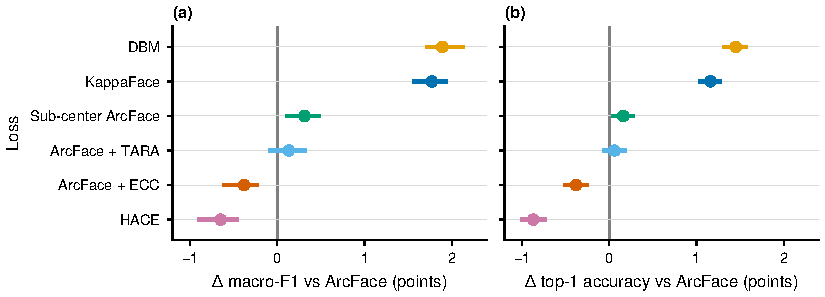
\includegraphics[width=\linewidth]{figs/fig_loss_gaps.pdf}
\caption{\textbf{Only the two per-species-margin losses beat ArcFace by more than a
fraction of a point.} Each row is one loss; the dot is its score minus ArcFace's score,
in percentage points, for (a) macro-F1 and (b) top-1 accuracy. A dot right of the
vertical line means the loss beats ArcFace. The horizontal bar is the 95\% interval from
a paired bootstrap over validation images, so it reflects which images are in the
validation set but not seed-to-seed variation; seed-to-seed variation, measured for
DBM, KappaFace and ArcFace, is about 0.1 points or less. Full validation set, seed 42.
X2-Softmax ($-48$ points of macro-F1, $-45$ of accuracy) is off the scale.}
\label{fig:gaps}
\end{figure}

\paragraph{DBM and KappaFace win, and are nearly tied.} Both beat ArcFace by 1.2--1.5
points of accuracy and 1.8--1.9 points of macro-F1. Changing the seed moves any of the
three retrained losses by about 0.1 points or less, so these gaps are 20 to 40 times
larger than the seed-to-seed variation. Between the two winners, DBM is ahead in both
seeds, by 0.29 points of accuracy each time and by 0.11 and 0.14 points of macro-F1. On
macro-F1 this difference is small: the bootstrap interval for KappaFace minus DBM,
$[-0.36, +0.02]$, just includes zero, so we read the two as close to a tie on our main
metric. DBM also has the best top-5 accuracy (0.962). It has a practical advantage as
well: unlike KappaFace, whose per-species running statistics are not synchronised across
GPUs, it can be trained on two GPUs.

\paragraph{Sub-center ArcFace gives a small but real gain, and TARA has no detectable
effect.} Sub-center ArcFace improves on ArcFace by 0.16 points of accuracy and 0.31
points of macro-F1, and both intervals lie above zero. TARA's gains, 0.06 and 0.13
points, have intervals that include zero, so we cannot distinguish TARA from plain
ArcFace.

\paragraph{ECC and HACE are worse than ArcFace.} ECC loses 0.38 points on both metrics,
and HACE loses 0.87 points of accuracy and 0.65 of macro-F1. HACE shows an interesting
pattern, though. Its top-5 accuracy, 0.952, is higher than ArcFace's 0.947. In other
words, HACE more often places the correct species among its five best guesses, but less
often ranks it first.

\paragraph{X2-Softmax fails.} X2-Softmax reaches only 38\% accuracy. Its learning curve
rose slowly throughout training and did not level off, so it was still learning, only
far too slowly. A natural suspect was the scale: we used $s = 30$ for every head, while
the X2-Softmax paper uses $s = 64$. A rerun at $s = 64$ learned even more slowly, reaching
0.112 accuracy at epoch 6.8 and 0.140 at epoch 10.2, and we stopped it there. The scale
is therefore not the cause. The geometry analysis in Section~\ref{sec:res-geom} shows
what goes wrong instead: its features collapse.

\subsection{Per-species results and the role of training-set size}
\label{sec:res-fine}

Overall macro-F1 is an average over all species, and an average can hide where a gain
comes from. In this section we look at the F1 score of each species separately. A
species' F1 is the harmonic mean of its precision (of the images the model labelled as
this species, the fraction that really were) and its recall (of this species' images,
the fraction the model found). We then group species by how many training images they
have. Although Herbarium 2022 caps species at 73 training images, there is still a rare
tail: 1{,}060 species have 10 or fewer. Figure~\ref{fig:count}a shows the mean
per-species F1 of each loss in each group. Figure~\ref{fig:count}b shows the gain over
ArcFace, computed species by species and then averaged within each group. Its intervals
come from a bootstrap that resamples the \emph{species} in each group (rather than the
images), and again do not include seed variation.

\begin{figure}[t]
\centering
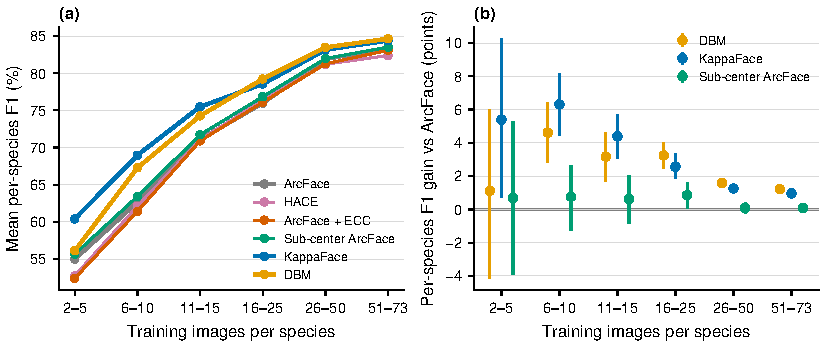
\includegraphics[width=\linewidth]{figs/fig_f1_by_count.pdf}
\caption{\textbf{DBM and KappaFace gain most on rare species; KappaFace leads on the
rarest.} Species are grouped into bands by their number of training images; the bands
hold 104 / 956 / 937 / 1{,}554 / 3{,}710 / 8{,}073 species, left to right. (a) For each
loss, the average F1 score of the species in each band (ArcFace + TARA is omitted
because it overlaps ArcFace). (b) For each species, the loss's F1 minus ArcFace's F1 on
the same species, averaged within each band; above zero means the loss does better than
ArcFace. Whiskers are 95\% intervals from resampling the species in each band, so they
are widest for the small 2--5 band, and they do not include seed-to-seed variation.
Seed 42, full validation set; the 167 species with no validation images are excluded.}
\label{fig:count}
\end{figure}

\paragraph{The gains are concentrated in the rare tail.} For species with 6--10
training images, KappaFace improves per-species F1 over ArcFace by 6.3 points and DBM by
4.6 points. For species with 51--73 images, which make up more than half of all species,
both add only about 1 point (KappaFace 1.0, DBM 1.2). Sub-center ArcFace adds less than
1 point in every group. This matches what the two winning losses are designed to do,
since both put larger margins on rare species.

\paragraph{Rare species remain much harder for every loss.} Even the best loss in each
group is about 24 points worse on species with 2--5 training images (KappaFace, 60.4)
than on species with 51--73 (DBM, 84.6). The better losses narrow this gap but are far
from closing it.

\paragraph{Fewer species are never recognised.} A species has an F1 of zero when the
model never predicts it correctly for any of its validation images. The number of such
species falls from 367 with ArcFace to 313 with DBM and 255 with KappaFace.

\paragraph{No loss changes the kind of mistake.} For every loss that trained properly,
75--78\% of wrong answers still name a species in the correct genus, and 87--90\% one in
the correct family (for example, 75.5\% and 87.7\% for ArcFace, and 77.8\% and 89.5\% for
DBM). The better losses therefore make fewer mistakes, but not different ones. Even
HACE, which is built around the taxonomy, does not shift this pattern.

\paragraph{KappaFace and DBM win on different species.} Figure~\ref{fig:crossover}
compares the two winners directly, species by species, using both seed pairs. KappaFace
is better on species with fewer than about 10 training images: by 3.4 points for
species with 2--5 images and 2.9 points for 6--10, with intervals above zero when both
seeds are pooled. The two tie for species with 11--15 images. From 16 images upward,
DBM is better, by 0.9, 0.4 and 0.2 points in the three remaining groups. These groups
contain most of the species, which is why overall macro-F1 barely separates the two
losses: KappaFace's large gains on a few rare species are offset by DBM's small gains on
many common ones. This crossover was measured on Herbarium 2022. It does not reappear on
the larger ladder data, where KappaFace trails DBM in every group
(Section~\ref{sec:res-ladder}).

\begin{figure}[t]
\centering
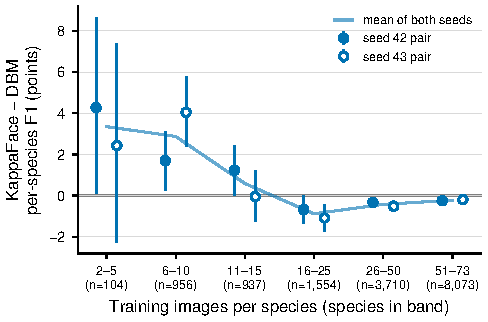
\includegraphics[width=3.25in]{figs/fig_crossover.pdf}
\caption{\textbf{KappaFace beats DBM on rare species, DBM wins on common ones.}
For each species, KappaFace's F1 minus DBM's F1, averaged within each band of training
images; above zero means KappaFace does better. The comparison is made twice, once
between the two seed-42 models (filled) and once between the two seed-43 models (open).
Whiskers are 95\% intervals from resampling the species in each band; the line is the
average of the two seed comparisons. The sign agrees across seeds in every band except
11--15, where the two losses tie.}
\label{fig:crossover}
\end{figure}

\paragraph{Combining the two winners without retraining.} Because the two losses win on
different species, we tested a simple way to combine them at prediction time. For each
image, we look at the species KappaFace predicts. If that species has at most $T$
training images, we keep KappaFace's answer; otherwise we use DBM's. To avoid tuning on
the same images we report on, we chose $T$ on a random half of the validation images
($T = 12$ for the seed-42 pair and $T = 10$ for the seed-43 pair) and scored the
combined model on the other half (Table~\ref{tab:routing}). This routing raises F1 on the
rarest species by 3--8 points while leaving common species within $\pm 0.1$ points. Only
1.4--2.2\% of images end up using KappaFace's answer, so the overall macro-F1 gain is
small, $+0.14$ points, about the size of the seed-to-seed variation. The real benefit is
for rare species, and the cost is running two models at prediction time. Whether this gain
is specific to KappaFace is tested on the ladder in Section~\ref{sec:res-routing}, and
largely it is not.

\begin{table}[t]
\centering
\small
\caption{\textbf{Routing rare-species predictions to KappaFace lifts the tail.} Scores
on the held-out validation half, with $T$ chosen on the other half. Accuracy and
macro-F1 are fractions; band columns are mean per-species F1.}
\label{tab:routing}
\footnotesize
\begin{tabular}{@{}llcccc@{}}
\toprule
Seed pair & Model & Top-1 & Macro-F1 & F1, 2--5 imgs & F1, 6--10 imgs \\
\midrule
\multirow{3}{*}{42 ($T=12$)} & DBM       & 0.8449 & 0.8078 & 0.517 & 0.672 \\
                             & KappaFace & 0.8426 & 0.8076 & 0.571 & 0.685 \\
                             & Routed    & \textbf{0.8456} & \textbf{0.8092} & \textbf{0.594} & \textbf{0.700} \\
\midrule
\multirow{3}{*}{43 ($T=10$)} & DBM       & 0.8458 & 0.8104 & 0.541 & 0.657 \\
                             & KappaFace & 0.8425 & 0.8061 & 0.566 & 0.686 \\
                             & Routed    & \textbf{0.8463} & \textbf{0.8118} & \textbf{0.591} & \textbf{0.708} \\
\bottomrule
\end{tabular}
\end{table}

\subsection{Representation geometry}
\label{sec:res-geom}

Accuracy tells us how often a model is right, but not what its feature space looks like.
To see whether the losses organise the feature space differently, we saved the
1{,}024-dimensional feature of every validation image for every model and computed the
same geometry measures as in the earlier CE-versus-ArcFace study. All of them are based
on each species' \emph{centroid}, the average feature of its validation images.

The \emph{within-species cosine} is the average cosine between an image's feature and
its own species' centroid. Higher values mean that images of the same species point in
more similar directions, so each species forms a tighter cluster. The
\emph{nearest-species cosine} is the cosine between each species' centroid and the
closest centroid of any other species, averaged over species. Lower values mean that even
the most similar neighbouring species is further away. The \emph{separation gap} is the
first minus the second. A large gap means clusters are tight compared with how close
their nearest neighbour is. A gap near zero means a typical image sits no closer to its
own species' centre than that centre sits to the nearest other species' centre. \emph{NC1} compares the spread of features
within each species with the spread between species centroids, so lower values again mean
tighter, better separated clusters. Finally, the \emph{alignment} is the cosine between
each species' weight vector (its template in the classifier) and its feature centroid.
High alignment means the classifier's template points straight at where that species'
images actually land. By the usual reading, a higher gap, higher alignment and lower NC1
all indicate ``tidier'' geometry. Results are in Table~\ref{tab:geom} and
Figure~\ref{fig:geom}. The seed-43 retrains of DBM, KappaFace and ArcFace reproduce
every value to within 0.003, so these measures are stable.

\begin{table}[t]
\centering
\small
\caption{\textbf{Geometry of the 384\,px models} (full validation set, seed 42). The
last column is the within-model Spearman correlation between per-species alignment and
per-species recall.}
\label{tab:geom}
\footnotesize
\setlength{\tabcolsep}{4pt}
\begin{tabular}{@{}lccccccc@{}}
\toprule
Loss & Within & Nearest & Gap & NC1 & Align. & $\rho$(align, recall) & Macro-F1 \\
\midrule
DBM                & 0.721 & 0.667 & 0.055 & 0.108 & 0.694 & 0.44 & \textbf{0.8161} \\
KappaFace          & 0.733 & 0.622 & 0.111 & 0.089 & 0.763 & 0.45 & 0.8150 \\
Sub-center ArcFace & 0.773 & 0.532 & 0.241 & 0.063 & 0.795 & 0.38 & 0.8003 \\
ArcFace + TARA     & 0.779 & 0.543 & 0.236 & 0.061 & 0.839 & 0.43 & 0.7986 \\
ArcFace            & 0.772 & 0.530 & 0.242 & 0.062 & 0.838 & 0.44 & 0.7972 \\
ArcFace + ECC      & 0.786 & 0.524 & \textbf{0.261} & \textbf{0.056} & \textbf{0.840} & 0.39 & 0.7934 \\
HACE               & 0.684 & 0.661 & 0.023 & 0.142 & 0.474 & 0.46 & 0.7908 \\
X2-Softmax         & 0.992 & 0.993 & $-$0.001 & 0.017 & 0.610 & $-$0.10 & 0.3136 \\
\bottomrule
\end{tabular}
\end{table}

\begin{figure}[t]
\centering
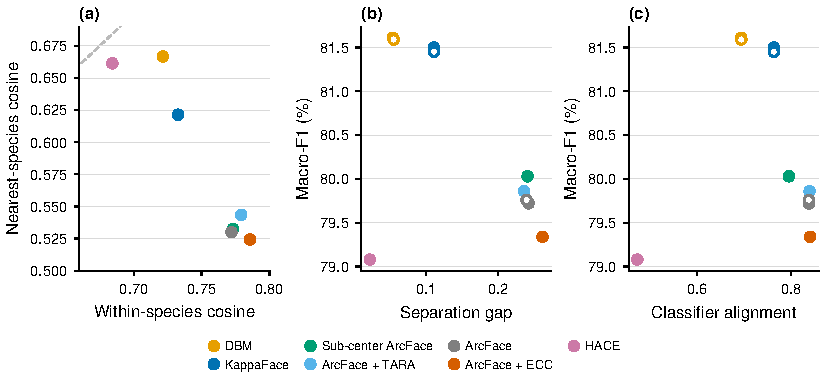
\includegraphics[width=\linewidth]{figs/fig_geometry.pdf}
\caption{\textbf{The two best losses have looser geometry than every ArcFace-family
loss.} Each point is one model, with every measure averaged over the 15{,}334 validation
species. (a) Horizontal axis: how tight each species' cloud is, the average cosine
between an image's feature and its own species' centroid (higher is tighter). Vertical
axis: how close the nearest other species is, the cosine between each species' centroid
and the closest other centroid (higher is closer). On the dashed diagonal the two are
equal, meaning a typical image sits no closer to its own species' centre than that
centre sits to its neighbour's centre. Points further below the diagonal have tighter
clouds with more distant neighbours. DBM and KappaFace sit closer to the diagonal than
any ArcFace-family loss; only HACE is closer. (b) Macro-F1 against the separation gap,
the horizontal minus the vertical value in (a). (c) Macro-F1 against alignment, the
average cosine between each species' classifier weight vector and its centroid. Filled
markers are seed 42; open markers are the seed-43 retrains, which land on top of them.
X2-Softmax (macro-F1 31\%, collapsed features) is off the scale.}
\label{fig:geom}
\end{figure}

\paragraph{Across losses, tidier average geometry goes with lower macro-F1.} This is the
opposite of what one might expect. The two best losses, DBM and KappaFace, have the
smallest separation gaps of any loss that trained properly apart from HACE: 0.055 and
0.111, against 0.242 for ArcFace. Their alignment is also lower, 0.69 and 0.76 against
0.84. In Figure~\ref{fig:geom}a, they sit closer than any ArcFace-family loss to the
diagonal, where a typical image is no closer to its own species' centre than that centre
is to the nearest other species' centre. At the other end, ECC has
the tidiest geometry of any loss on all three measures, yet the lowest macro-F1 of the
ArcFace family. Combined with the earlier CE-to-ArcFace result, where geometry improved
greatly but accuracy only a little, this tells us that average geometry is not a reliable
target for choosing a loss on this data. One possible reading, which we have not yet
tested, is that the averages are dominated by the many common species, whose clusters
ArcFace-style losses make very neat, while DBM and KappaFace spend their effort on rare
species instead.

\paragraph{Within a single model, geometry still predicts which species are recognised.}
Although geometry does not rank the losses, it remains informative inside each model.
For every loss, species whose template is better aligned with their cluster have higher
recall. The Spearman rank correlation between per-species alignment and per-species
recall is 0.38--0.46 across models (last column of Table~\ref{tab:geom}).

\paragraph{X2-Softmax's features have collapsed.} For X2-Softmax, the within-species and
nearest-species cosines are both about 0.99. Almost every image's feature points in
nearly the same direction, regardless of species, so the model has to separate 15{,}501
species inside a very narrow cone of directions. This is consistent with how slowly and
poorly it learned.

\paragraph{HACE's species templates are poorly aligned.} HACE has the lowest alignment
of the working losses, 0.47. This needs care in interpretation: HACE's classifier also
has outputs for genera and families, and its prediction combines information across the
whole tree, so its species templates alone describe only part of the model.

\subsection{Scaling ladder}
\label{sec:res-ladder}

\begin{table}[t]
\centering
\small
\caption{\textbf{The order is the same on every rung: DBM, then KappaFace, then
ArcFace.} Final top-1 accuracy / macro-F1 after 131{,}250 steps, on the full validation
set of each rung, one seed per run. The last two columns give each loss's score minus
ArcFace's (its ``lead''), in points.}
\label{tab:ladder}
\footnotesize
\setlength{\tabcolsep}{2pt}
\begin{tabular}{@{}lccccc@{}}
\toprule
Rung (epochs) & DBM & KappaFace & ArcFace & DBM lead & KappaFace lead \\
\midrule
15.5k (24.6) & 0.8959 / 0.8436 & 0.8909 / 0.8329 & 0.8842 / 0.8178 & $+1.17$ / $+2.58$ & $+0.67$ / $+1.51$ \\
32k (20.1)   & 0.8882 / 0.7754 & 0.8835 / 0.7597 & 0.8777 / 0.7452 & $+1.05$ / $+3.02$ & $+0.58$ / $+1.45$ \\
64k (14.9)   & 0.8619 / 0.6818 & 0.8565 / 0.6592 & 0.8490 / 0.6429 & $+1.29$ / $+3.89$ & $+0.75$ / $+1.63$ \\
\bottomrule
\end{tabular}
\end{table}

\begin{figure}[t]
\centering
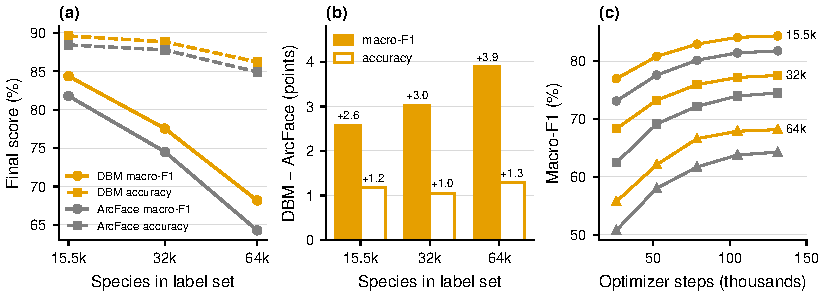
\includegraphics[width=\linewidth]{figs/fig_ladder.pdf}
\caption{\textbf{DBM's macro-F1 lead over ArcFace grows as rare species are added;
KappaFace's does not.} (a) Final macro-F1 (solid lines) and top-1 accuracy (dashed lines)
of DBM (orange), KappaFace (blue) and ArcFace (grey) on the three nested label sets; the
horizontal axis is logarithmic in the number of species. (b) Each loss's score minus
ArcFace's at the end of training, in percentage points, for macro-F1 (solid) and accuracy
(dashed). (c) Macro-F1 lead over ArcFace at each of the five evaluations during training,
one every 26{,}250 steps; colours as in (a), with one marker shape per label set (circles
15.5k, squares 32k, triangles 64k; the orange lines are labelled at their left end). Every
run trains for the same 131{,}250 steps, so larger label sets get fewer epochs. Single
seed per run; seed-to-seed variation at 15k was about 0.1 points.}
\label{fig:ladder}
\end{figure}

Table~\ref{tab:ladder} and Figure~\ref{fig:ladder} give the results of the ladder.

\paragraph{The ranking holds at every size.} On all three rungs, DBM is first, KappaFace
second and ArcFace third, on both top-1 accuracy and macro-F1. This is the same order as
on Herbarium 2022 (Table~\ref{tab:main}).

\paragraph{DBM's macro-F1 lead grows with the number of species, but KappaFace's does
not.} DBM's macro-F1 lead over ArcFace increases from 2.6 points at 15.5k to 3.0 at 32k
and 3.9 at 64k, while its accuracy lead stays roughly flat at 1.0--1.3 points.
KappaFace's macro-F1 lead is essentially flat, at about 1.5, 1.5 and 1.6 points, and its
accuracy lead is 0.6--0.8 points. As a result, DBM's advantage over KappaFace itself
grows, from 1.1 to 1.6 to 2.3 points of macro-F1. The difference between the two metrics
follows from how the rungs are built and how the metrics weight species. The larger rungs
mostly add rare species (Table~\ref{tab:ladder-data}): the median number of training
images per species falls from 57 to 20 to 10. Rare species contribute few images, so they
barely affect accuracy, but each one counts as much as any other species in macro-F1.
This matches the 15k per-species result, where DBM's gains were largest for rare species.
Why DBM's lead grows while KappaFace's does not is not something these runs explain.

\paragraph{Adding species costs much more macro-F1 than accuracy.} Going from 15.5k to
64k species, DBM's macro-F1 drops from 0.844 to 0.682, KappaFace's from 0.833 to 0.659
and ArcFace's from 0.818 to 0.643. Accuracy drops much less: from 0.896 to 0.862 for DBM,
0.891 to 0.857 for KappaFace and 0.884 to 0.849 for ArcFace. The species added at each
step are hard to learn from so few images, but because they have few images they hardly
register in accuracy.

\paragraph{The lead appears early and narrows.} At the first evaluation, after 20\% of
training, DBM already leads ArcFace by 3.9, 5.9 and 5.0 points of macro-F1 on the three
rungs, and KappaFace leads by 2.2, 2.2 and 1.7. DBM's lead shrinks over training, though
not steadily (at 64k it rises briefly at the third evaluation), and it never closes
(Figure~\ref{fig:ladder}c). KappaFace's lead shrinks less. All three losses are still
improving slowly at the end of training, most visibly on the 64k rung, which gets the
fewest passes over its data.

\paragraph{KappaFace's rare-species advantage does not appear on the ladder.}
Figure~\ref{fig:ladder-bands} repeats, on the ladder, the species-by-species comparison of
Figure~\ref{fig:crossover}. Here KappaFace is behind DBM in every group of training-image
counts on every rung, and in all 21 cases (three rungs times seven groups) the 95\%
interval lies below zero. The gap is largest for the rarest species and grows with the
number of species: for species with 2--5 training images it is $-4.2$ points at 32k and
$-5.7$ at 64k. At 15.5k it is $-15.1$ points, but that group holds only 31 species, so the
estimate is very noisy (interval $-30.1$ to $-2.2$). For species with 101 or more training
images the gap is about $-0.2$ to $-0.3$ points. Why the crossover seen on Herbarium 2022
disappears on this data is not yet known. The ladder's training set is larger and more
imbalanced than the ablation's, but we have not tested which difference matters.

\begin{figure}[t]
\centering
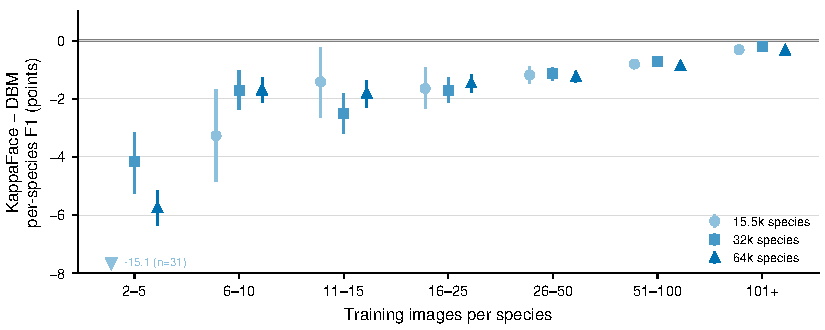
\includegraphics[width=\linewidth]{figs/fig_ladder_bands.pdf}
\caption{\textbf{On the ladder, KappaFace is behind DBM in every training-image group.}
For each species, KappaFace's F1 minus DBM's F1, averaged within each group of species
defined by their number of training images; below zero means KappaFace does worse. One
marker shape per rung (circles 15.5k, squares 32k, triangles 64k). The 2--5 group holds
31, 4{,}593 and 13{,}738 species on the three rungs. Whiskers are 95\% intervals from
resampling the species in each group, and do not include seed-to-seed variation. The
15.5k point in the 2--5 group ($-15.1$, 31 species, interval $-30.1$ to $-2.2$) is off
the scale and is shown by the arrow. Compare Figure~\ref{fig:crossover}, where the sign is
reversed for the rarest groups on Herbarium 2022. One seed per loss.}
\label{fig:ladder-bands}
\end{figure}

\paragraph{Caveats.} Each ladder point comes from a single seed. The seed-to-seed
variation we measured at 15k was about 0.1 points, far below these gaps, but it was
measured on different data. Every rung gets the same compute, so the larger rungs are
trained for fewer epochs, and with more training part of the gap between rungs might
close. On the 64k rung the median species has only 3 validation images, so the F1 score
of any individual species there is very noisy, even though the average over tens of
thousands of species is stable. Finally, the validation sets change in composition from
rung to rung. All images of the added species come from Herbarium 2021, so the share of
2021 images in the validation set rises from 58\% to 65\% to 74\%
(Table~\ref{tab:ladder-data}), and 2021 images are easier to classify than 2022 images
(Section~\ref{sec:res-data}). We have not measured how much this shift affects the
cross-rung trend in macro-F1.

\subsection{Combining two models on the ladder}
\label{sec:res-routing}

Section~\ref{sec:res-fine} showed that sending KappaFace's answer to rare species helps on
Herbarium 2022. We repeat that test on the ladder, again with no retraining. As before, for
each image we look at the species KappaFace predicts. If that species has at most $T$
training images, we use KappaFace's answer, and otherwise DBM's. The cutoff $T$ is chosen
on one random half of the validation images, and the rule is scored on the other half. We
call this \emph{routing}. Table~\ref{tab:ladder-routing} gives the result.

\begin{table}[t]
\centering
\small
\caption{\textbf{Routing rare-species answers to KappaFace helps on every rung, and more on
larger label sets.} Scores on the held-out half of each rung's validation set, with the
cutoff $T$ chosen on the other half. Top-1 accuracy / macro-F1. ``Images using KappaFace's
answer'' counts every image where KappaFace's top answer names a species with at most $T$
training images, including images where the two models agree.}
\label{tab:ladder-routing}
\footnotesize
\setlength{\tabcolsep}{4pt}
\begin{tabular}{@{}lcccccc@{}}
\toprule
Rung & $T$ & Images using & DBM alone & Routed & Change (points) \\
 & & KappaFace's answer & & & \\
\midrule
15.5k & 20 & 2.1\% & 0.8952 / 0.8364 & 0.8958 / 0.8402 & $+0.06$ / $+0.38$ \\
32k   & 10 & 2.5\% & 0.8883 / 0.7879 & 0.8892 / 0.7933 & $+0.09$ / $+0.54$ \\
64k   & 8  & 3.0\% & 0.8621 / 0.7033 & 0.8634 / 0.7100 & $+0.13$ / $+0.67$ \\
\bottomrule
\end{tabular}
\end{table}

\paragraph{Routing helps on every rung, and more as species are added.} Macro-F1 rises
by 0.38, 0.54 and 0.67 points at 15.5k, 32k and 64k, and accuracy by 0.06 to 0.13 points.
The gain is concentrated in the rare groups. At 64k, F1 for species with 2--5 training
images rises by 1.9 points and for species with 6--10 images by 2.5 points, while for
species with 26 or more training images it changes by at most 0.14 points. The per-species
gain in the rare groups is actually smaller on the larger rungs (for species with 6--10
training images it is 4.3, 3.4 and 2.5 points). The macro-F1 gain grows because rare
species make up a growing share of all species: 7\%, 33\% and 46\% of the validation
species on the three rungs have 10 or fewer training images. This is consistent with the
numbers, but we have not separated the two effects.

\paragraph{Why can routing help if KappaFace is worse on rare species?} The rule does not
send all rare species to KappaFace. It switches only when KappaFace's \emph{own answer}
names a rare species, that is, when KappaFace commits to a rare species. To see what this
does, we counted, image by image, how the rule changes DBM's answers on the full
validation sets of the 32k and 64k rungs. At 64k (with $T=8$), the rule changes 2{,}599 of
562{,}308 answers. Of these, 1{,}252 become correct, 513 become wrong (DBM had been right),
and 834 are wrong under both models, a net gain of 739 correct answers. At 32k (with
$T=10$), it changes 1{,}481 answers: 712 become correct, 334 become wrong and 435 are wrong
either way, a net gain of 378. Every one of the corrections at 64k is an image of a species
with at most 10 training images (469 with 2--5 and 783 with 6--10). This is expected,
because for KappaFace's answer to be correct it must name the true species, and the rule
only accepts answers that name rare species.

The 469 corrections for species with 2--5 training images at 64k are 469 images of 469
different species, with one validation image each, spread over 125 plant families. Each
family's share of these corrections is close to its share of the whole group (for example
Fabaceae 6.8\% against 6.5\%, and Orchidaceae 6.8\% against 6.4\%), so there is no set of
``KappaFace species''. On these images, DBM's wrong answer is in the same genus as the true
species 61\% of the time and in the same family 80\% of the time, and the species it chose
has a median of 27 training images, against 2--5 for the true species. Our reading, not
tested, is that DBM sometimes leans toward a better-known sister species where KappaFace
does not.

\begin{figure}[t]
\centering
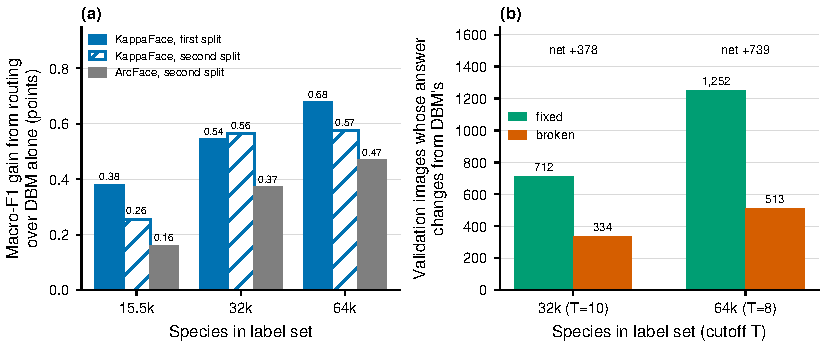
\includegraphics[width=\linewidth]{figs/fig_routing.pdf}
\caption{\textbf{Most of the routing gain does not need KappaFace.} (a) Macro-F1 gain, in
points, from using the second model's answer when it names a rare species, relative to DBM
alone, on the held-out half of each validation set. Solid blue: KappaFace as the second
model, first analysis. Hatched blue: KappaFace again, in a repeat analysis that drew its
own random halves, so the difference between the two blue bars is split-to-split
variation. Grey: plain ArcFace as the second model in the repeat analysis, on the same
halves as the hatched bars. The cutoff $T$ is chosen separately for each bar, on the other
half. (b) How routing changes DBM's answers on the full validation set at 32k and 64k:
``fixed'' answers were wrong and become right, ``broken'' answers were right and become
wrong. Answers that are wrong under both models (435 and 834) are not shown. One seed per
model, and no uncertainty interval on the gains.}
\label{fig:routing}
\end{figure}

\paragraph{A control: most of the gain comes from combining any two different models.}
To test whether the gain is specific to KappaFace, we repeated the rule with plain
ArcFace as the second model. ArcFace is the weakest of the three models on its own. This
repeat analysis drew its own random halves, so its DBM-alone scores differ slightly from
Table~\ref{tab:ladder-routing} (for example 0.8378 against 0.8364 macro-F1 at 15.5k);
within it, KappaFace and ArcFace are compared on the same halves. With KappaFace as the
second model, macro-F1 rises by 0.26, 0.56 and 0.57 points on the three rungs. With ArcFace
it rises by 0.16, 0.37 and 0.47 points, which is 62\%, 65\% and 81\% of KappaFace's gain
(Figure~\ref{fig:routing}a). Among the images where the rule changes the answer, the
second model is right 37--45\% of the time with ArcFace and 40--47\% with KappaFace,
against 22--26\% for DBM on the same images. So even a model that is worse than DBM overall
is more often right than DBM on the answers it contributes. KappaFace adds a little more
than ArcFace (0.10, 0.19 and 0.10 points of macro-F1), but this is about the size of the
split-to-split variation: KappaFace's own gains differ between the two analyses by up to
0.12 points. We therefore cannot say that KappaFace is better than ArcFace as the second
model.

\paragraph{Caveats.} One seed per model, and no uncertainty interval on the routing
gains. Routing needs two models at prediction time. The ArcFace control was run only on
the ladder, so we do not know how much of the Herbarium 2022 routing gain
(Section~\ref{sec:res-fine}) is generic in the same way.

\subsection{Checks on the data}
\label{sec:res-data}

Two properties of the data affect how the numbers above should be read. First, the ladder's
15.5k set has the same species as the Herbarium 2022 ablation but much higher scores (DBM
reaches 0.844 macro-F1 there, against 0.816 in the ablation). Second, herbarium collections
can hold more than one image of the same physical specimen, so a validation image can have
a near-identical twin in the training set.

\paragraph{Why the ladder scores higher than the ablation.} The ladder's validation set is
a mixture. Of its 341{,}932 images, 197{,}180 (58\%) come from Herbarium 2021, 115{,}659
(34\%) are Herbarium 2022 training images that the merged data happened to place in
validation, and 29{,}093 (9\%) are original Herbarium 2022 validation images. The DBM
model scores very differently on these parts (Table~\ref{tab:datacheck}, block A): 0.933
accuracy on the 2021 part, against about 0.85 on the two 2022 parts. A fair comparison with
the ablation therefore uses only the 29{,}093 original 2022 validation images, which
neither the ladder model nor the ablation models trained on (block B). On this common
subset, ladder DBM scores 0.848 accuracy and 0.794 macro-F1, against 0.845 and 0.789 for
the ablation's DBM. So doubling the training data helped only a little, about 0.4 points on
both metrics, and the large headline difference comes from the easier validation images.
Within a rung, every loss is scored on the same images, so comparisons between losses are
fair.

\begin{table}[t]
\centering
\small
\caption{\textbf{The ladder's Herbarium 2021 validation images are much easier, and on the
images the two setups share, ladder DBM is only slightly ahead of the ablation's DBM.}
Top-1 accuracy / macro-F1. (A) Ladder 15.5k DBM on the three parts of its validation set.
(B) The 29{,}093 images from the original 2022 validation set (12{,}352 species), which no
model here trained on. Macro-F1 values in different rows of block A cover different sets
of species and are not directly comparable.}
\label{tab:datacheck}
\footnotesize
\begin{tabular}{@{}llrc@{}}
\toprule
 & Model and validation images & Images & Top-1 / macro-F1 \\
\midrule
A & Ladder DBM, images from Herbarium 2021 & 197{,}180 & 0.9325 / 0.8384 \\
  & Ladder DBM, images from the 2022 training split & 115{,}659 & 0.8455 / 0.8168 \\
  & Ladder DBM, images from the 2022 validation split & 29{,}093 & 0.8484 / 0.7936 \\
  & Ladder DBM, all & 341{,}932 & 0.8959 / 0.8436 \\
\midrule
B & Ladder 15.5k DBM & 29{,}093 & 0.8484 / 0.7936 \\
  & Ablation DBM, seed 42 & 29{,}093 & 0.8448 / 0.7892 \\
  & Ablation DBM, seed 43 & 29{,}093 & 0.8437 / 0.7863 \\
  & Ablation KappaFace & 29{,}093 & 0.8415 / 0.7852 \\
  & Ablation ArcFace & 29{,}093 & 0.8294 / 0.7702 \\
\bottomrule
\end{tabular}
\end{table}

\paragraph{Why are the 2021 images easier?} We do not yet know. Same-specimen copies, which
we measure next, do not explain it: 2021 images with no copy in the training set still
score 0.931. One untested guess is that they come mostly from species with many training
images.

\paragraph{Same-specimen copies.} To measure how often a validation image has a copy of the
same specimen in the training set, we used a generic image model that was not trained on
herbarium sheets (a SWIN-Base pretrained on ImageNet-22k, at 224\,px). We embedded every
training and validation image, and for each validation image we found the most similar
training image of the same species, measured by the cosine between the two embeddings. We
then looked at example pairs at different similarity levels (Figure~\ref{fig:neardup}) and
judged by eye that a similarity of about 0.93 or more means the same physical specimen:
identical scans at 0.99 and above, and re-scans or re-crops of the same sheet below that.
Below about 0.93 the pairs are different specimens that merely look alike. The 0.93
threshold is therefore a judgement from example pairs, not a calibrated value.

\begin{figure}[!tb]
\centering
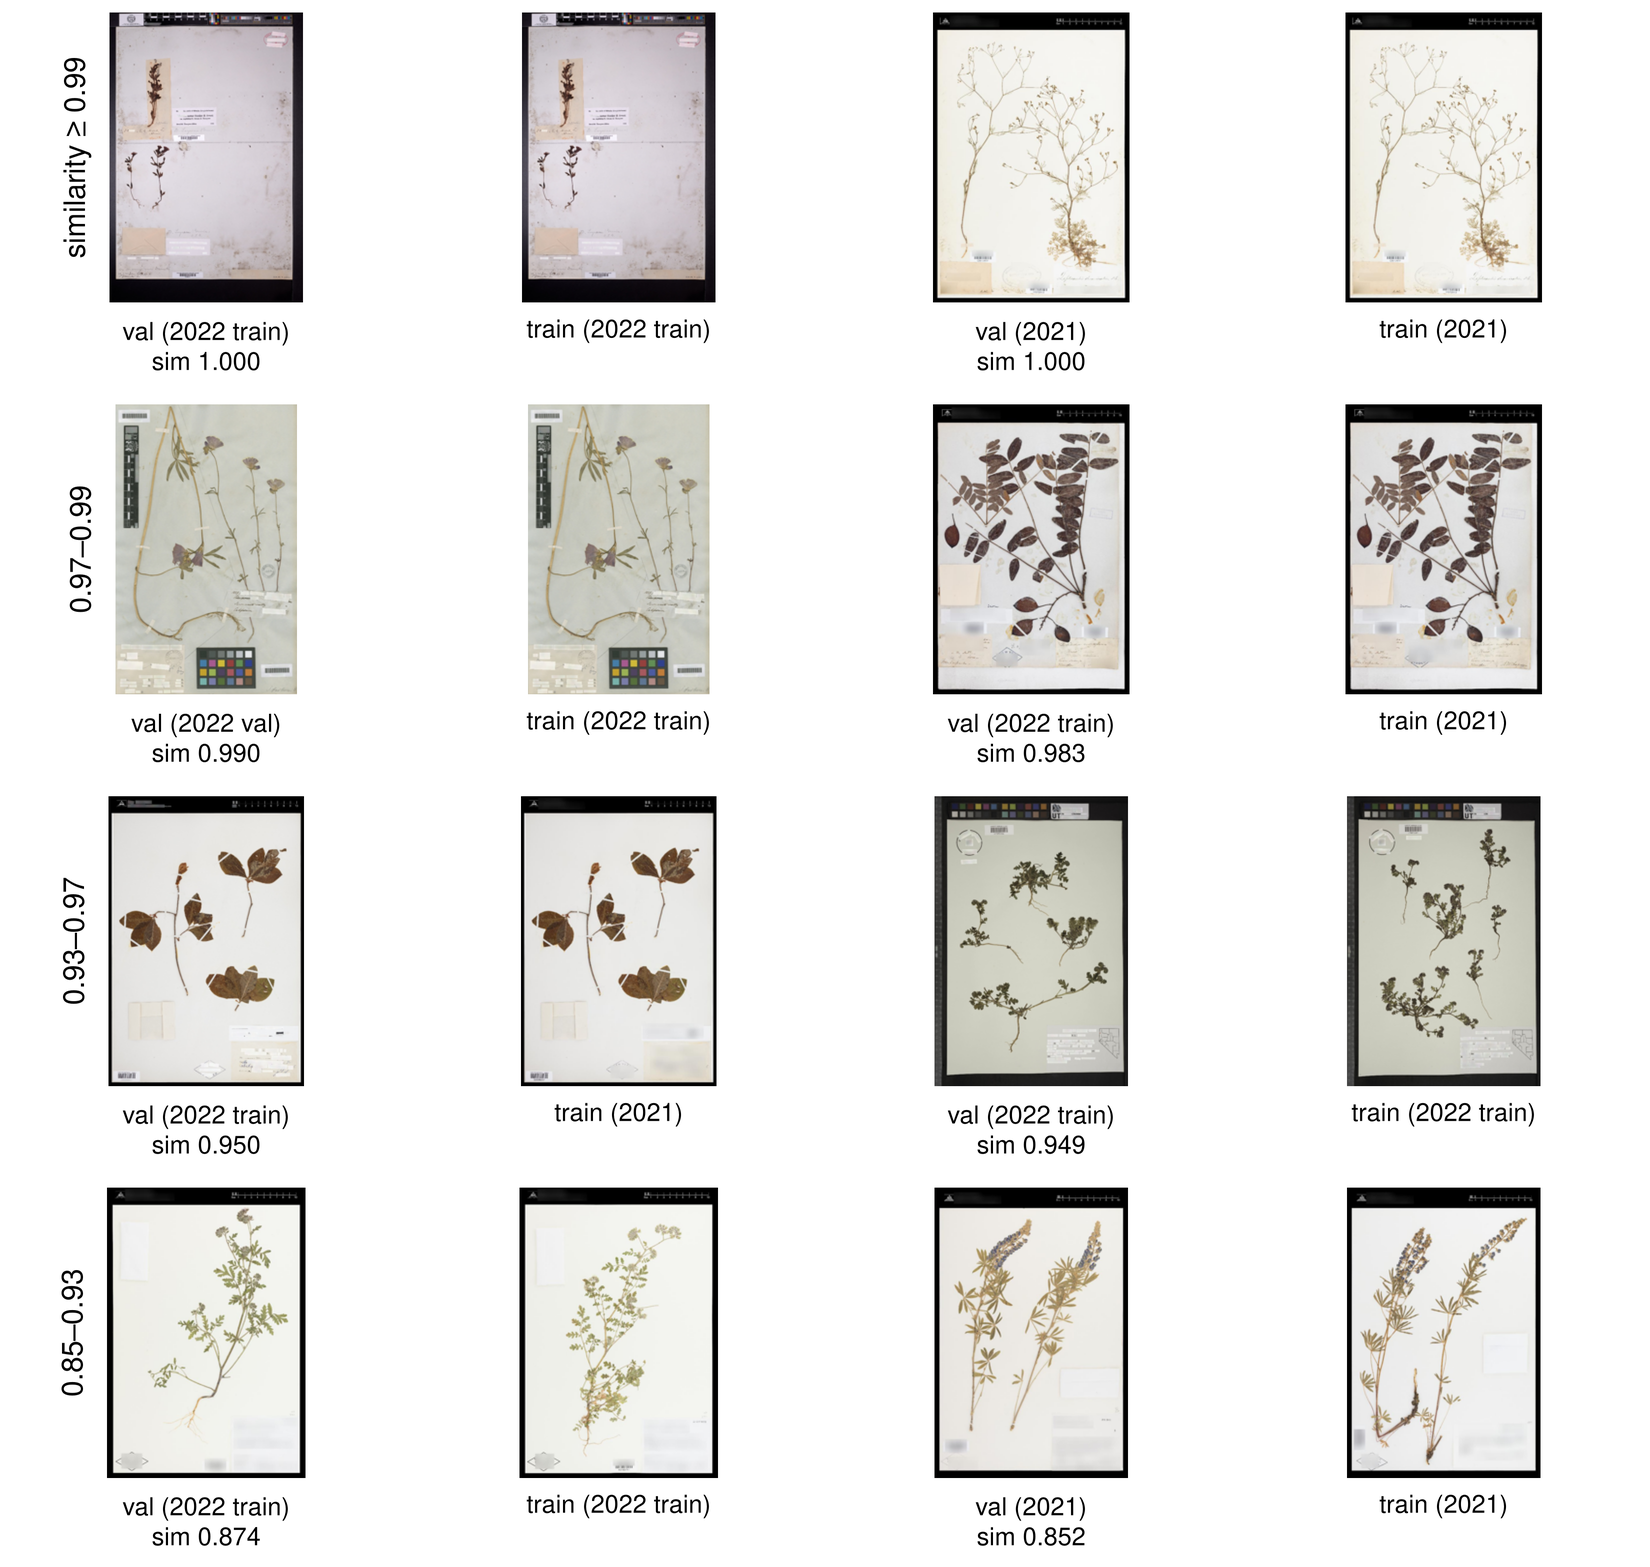
\includegraphics[width=0.8\linewidth]{figs/near_duplicate_examples.png}
\caption{\textbf{A similarity of about 0.93 or more means the same physical specimen.}
Each row shows two examples of a validation image (left of each pair) beside the most
similar training image of the same species (right), found with a generic ImageNet-22k
SWIN-Base. Rows are similarity bands, from identical scans (0.99 and above) to different
specimens that merely look alike (0.85--0.93). Labels give each image's source collection
in the original competitions, and the similarity. The threshold of about 0.93 was chosen by
looking at pairs like these.}
\label{fig:neardup}
\end{figure}

Table~\ref{tab:copies} gives the results. In the ablation data, 1.7\% of validation images
have a copy of the same specimen in the training set, and DBM gets 98\% of those right,
against 84\% of the rest. Because they are only 1.7\% of the images, they add about a
quarter of a point to overall accuracy (1.7\% of the images times an accuracy difference of
14.5 points). Every loss is scored on the same images, so this shifts all of them about
equally and the comparisons between losses stand, but absolute accuracy is slightly
inflated. The 1.7\% is a lower bound: only the 145{,}344 of 167{,}955 validation images that
survived into the merged data could be checked, and the merge had already removed exact
duplicates, so some copies may be missing. On the ladder, about 3\% of validation images
have a copy in the training set, and again the share is similar for the three image
sources, so the copies are not concentrated among the 2021 images. They add roughly 0.1 to
0.3 points to overall accuracy.

\begin{table}[t]
\centering
\small
\caption{\textbf{A few percent of validation images have a same-specimen copy in the
training set, and DBM gets nearly all of them right.} A copy means a same-species training
image with similarity of at least 0.93. The last column gives DBM's accuracy on validation
images with and without such a copy; the similarity threshold used there is in brackets
(0.95 for the ladder rows, the closest value measured for all of them).}
\label{tab:copies}
\footnotesize
\setlength{\tabcolsep}{4pt}
\begin{tabular}{@{}p{1.75in}rrp{1.2in}@{}}
\toprule
Validation images & Checked & With a copy ($\ge 0.93$) & DBM accuracy with / without \\
\midrule
Ablation: 2022 validation vs.\ 2022 training & 145{,}344 & 2{,}421 (1.7\%) & 0.983 / 0.838 ($\ge 0.93$) \\
Ladder 15.5k: from Herbarium 2021 & 197{,}180 & 6{,}104 (3.1\%) & 0.984 / 0.931 ($\ge 0.95$) \\
Ladder 15.5k: from the 2022 training split & 115{,}659 & 3{,}317 (2.9\%) & 0.984 / 0.843 ($\ge 0.95$) \\
Ladder 15.5k: from the 2022 validation split & 29{,}093 & 811 (2.8\%) & 0.979 / 0.846 ($\ge 0.95$) \\
\bottomrule
\end{tabular}
\end{table}

\paragraph{What this means for the results.} Neither check changes which loss wins, because
each loss is scored on the same validation images. They do mean that absolute accuracy is
slightly inflated by copies, that ladder scores should not be compared with the ablation
scores, and that part of any gain from combining models could in principle come from
recognising a near-identical training image. We have not measured that last point for the
routing corrections.

\section{Summary of findings so far}
\label{sec:summary}

The clearest result is that losses which give each species its own margin, DBM and
KappaFace, are the only interventions that improve on ArcFace by more than a fraction of
a point. They add about 1.9 points of macro-F1 and 1.2--1.5 points of accuracy, and the
gain holds with a second seed. Looking per species shows that these gains are
concentrated in the rare tail. On Herbarium 2022 the two losses divide that tail between
them: KappaFace is better below about 10 training images and DBM above about 15.

The other ideas we tested did not help as implemented. Using the taxonomy (HACE),
pulling features toward class centres (ECC) and aligning with BioCLIP (TARA) all
matched or fell below ArcFace, and no loss changed the share of errors that land in the
correct genus, which stays at 75--78\%. The geometry analysis adds a caution: across
losses, tidier average geometry did not mean higher accuracy, and the best losses have
looser species clusters than any ArcFace-family loss.

On the scaling ladder, the order is DBM, then KappaFace, then ArcFace at 15.5k, 32k and
64k species. DBM's macro-F1 lead over ArcFace grows as more, mostly rare, species are
added, from 2.6 to 3.9 points, while KappaFace's stays near 1.5 points. KappaFace's
advantage on the rarest species, seen on Herbarium 2022, does not reappear on the ladder.
Routing rare-species answers to KappaFace raises macro-F1 over DBM alone on every rung,
by 0.4 to 0.7 points in the first analysis. But a control with plain ArcFace as the second
model recovers 60--80\% of the gain, so most of it comes from combining two different
models, and we cannot say that KappaFace is special here.

Two checks on the data temper the absolute numbers but not the ranking of losses. About
1.7\% of the ablation's validation images, and about 3\% of the ladder's, have a copy of
the same physical specimen in the training set. And the ladder's validation set contains
many easier Herbarium 2021 images, which is why its 15.5k scores are higher than the
ablation's even though doubling the training data helped only about 0.4 points on the
images the two share.

\paragraph{Not yet measured.} Several pieces are still missing. Cross-entropy and
cross-entropy-with-logit-adjustment baselines at 384\,px on the Herbarium 2022 data are
training now and are not reported, so the comparison with the simplest baselines is still
missing. We do not know why the 2021 validation images are easier, why the KappaFace
crossover disappears on the ladder, or why DBM's lead grows with the number of species
while KappaFace's does not. The ArcFace control for routing was run only on the ladder,
routing gains have no uncertainty intervals, and we have not checked whether
KappaFace's routing corrections include same-specimen copies. Geometry has not been
split by rarity group, which would test the reading offered in Section~\ref{sec:res-geom},
and it has not been measured on the ladder models. FlexiGrad and the multi-task family,
genus and species heads have not been built. And apart from DBM, KappaFace and ArcFace on
Herbarium 2022, every run has used only one seed.

% Discussion intentionally left out of this draft.

\clearpage
\appendix
\section{Provenance}
\label{app:prov}

\begin{table}[t]
\centering
\small
\caption{Run identifiers behind each result (first 8 characters).}
\footnotesize
\begin{tabular}{@{}p{1.9in}p{3.3in}@{}}
\toprule
Result & Runs \\
\midrule
Full-set re-scores of the 8 losses & \texttt{f701e70f} \\
Training runs (seed 42) & ArcFace \texttt{6a899d4a}, sub-center \texttt{47362b64}, HACE \texttt{677aa821}, DBM \texttt{c2fecdb6}, X2 \texttt{0b103f18}, KappaFace \texttt{f13e6236}, ECC \texttt{8fff330a}, TARA \texttt{601daea1} \\
Seed-43 reruns & DBM \texttt{61e3b0a7} (re-score), KappaFace \texttt{cf97fa8d}, ArcFace \texttt{f4e0099f} \\
Per-species F1, bootstrap, error structure & \texttt{2964fe72} \\
KappaFace--DBM crossover and routing & \texttt{ab4f160f} \\
Geometry (11 models) & \texttt{bf50bd59} \\
X2-Softmax at $s=64$ & \texttt{877404ac} \\
224\,px references & CE \texttt{be436c7e}, ArcFace \texttt{be730cdf} / \texttt{da0667dc} \\
Ladder data build & \texttt{5c9db6fa} \\
Ladder final runs (DBM / KappaFace / ArcFace) & 15.5k \texttt{dc59af2e} / \texttt{0911811c} / \texttt{e3ecf637}, 32k \texttt{ca0355e1} / \texttt{2677643e} / \texttt{f30277ed}, 64k \texttt{29abd9c9} / \texttt{125ab8df} / \texttt{2244e684} \\
Ladder re-scores with saved predictions (DBM / KappaFace / ArcFace) & \texttt{a45f141b} / \texttt{f4d8caf9} / \texttt{54002e73} \\
Ladder per-group comparison and routing & \texttt{a8745409} \\
Routing, image-by-image counts; images behind the gain & \texttt{b9fbefe7}; \texttt{9ddce29c} \\
Routing control with ArcFace & \texttt{763995bb} \\
Ladder vs.\ ablation on the same images & \texttt{6c184416} \\
Same-specimen copies & \texttt{1eb2694b}, \texttt{4704f8f8} \\
In progress, not reported & CE \texttt{5a1a1645}, CE with logit adjustment \texttt{e2d28310} \\
\bottomrule
\end{tabular}
\end{table}

Figures are generated by \nolinkurl{figs/make_figures.py} from the data files in
\nolinkurl{figs/data/}.

\begin{thebibliography}{10}

\bibitem[Deng et al.(2019)]{arcface}
J.~Deng, J.~Guo, J.~Yang, N.~Xue, I.~Kotsia, and S.~Zafeiriou.
\newblock ArcFace: Additive angular margin loss for deep face recognition.
\newblock arXiv:1801.07698.
\newblock \url{https://www.alphaxiv.org/abs/1801.07698}

\bibitem[Deng et al.(2020)]{subcenter}
J.~Deng, J.~Guo, T.~Liu, M.~Gong, and S.~Zafeiriou.
\newblock Sub-center ArcFace: Boosting face recognition by large-scale noisy web
  faces.
\newblock In \emph{ECCV}, 2020.
\newblock \url{https://doi.org/10.1007/978-3-030-58621-8_43}

\bibitem[Oinar et al.(2023)]{kappaface}
C.~Oinar, B.~M. Le, and S.~S. Woo.
\newblock KappaFace: Adaptive additive angular margin loss for deep face
  recognition.
\newblock \emph{IEEE Access}, 2023. arXiv:2201.07394.
\newblock \url{https://www.alphaxiv.org/abs/2201.07394}

\bibitem[Xu et al.(2023)]{x2softmax}
J.~Xu, X.~Liu, X.~Zhang, Y.-W. Si, X.~Li, Z.~Shi, K.~Wang, and X.~Gong.
\newblock X2-Softmax: Margin adaptive loss function for face recognition.
\newblock arXiv:2312.05281.
\newblock \url{https://www.alphaxiv.org/abs/2312.05281}

\bibitem[Son et al.(2025)]{dbm}
M.~Son, I.~Koo, J.~Park, and C.~Kim.
\newblock Difficulty-aware balancing margin loss for long-tailed recognition.
\newblock In \emph{AAAI}, 2025.
\newblock \url{https://doi.org/10.1609/aaai.v39i19.34261}

\bibitem[Yao et al.(2024)]{ecc}
H.~Yao, Q.~Miao, P.~Zhao, C.~Li, X.~Li, G.~Feng, and R.~Liu.
\newblock Exploration of class center for fine-grained visual classification.
\newblock \emph{IEEE TCSVT}, 2024.
\newblock \url{https://doi.org/10.1109/tcsvt.2024.3406443}

\bibitem[Chan et al.(2026)]{hace}
A.~Chan, D.~D'Ascenzo, and S.~Cultrera di Montesano.
\newblock When labels have structure: Improving image classification with
  hierarchy-aware cross-entropy.
\newblock arXiv:2605.06274.
\newblock \url{https://www.alphaxiv.org/abs/2605.06274}

\bibitem[He et al.(2026)]{tara}
H.~He, Z.~Tan, and Y.~Peng.
\newblock Taxonomy-aware representation alignment for hierarchical visual
  recognition with large multimodal models.
\newblock arXiv:2603.00431.
\newblock \url{https://www.alphaxiv.org/abs/2603.00431}

\bibitem[Stevens et al.(2024)]{bioclip}
S.~Stevens, J.~Wu, M.~J. Thompson, E.~G. Campolongo, C.~H. Song, D.~E. Carlyn,
  W.-L. Chao, and Y.~Su.
\newblock BioCLIP: A vision foundation model for the tree of life.
\newblock In \emph{CVPR}, 2024.
\newblock \url{https://www.alphaxiv.org/abs/2311.18803}

\bibitem[Liu et al.(2021)]{swin}
Z.~Liu, Y.~Lin, Y.~Cao, H.~Hu, Y.~Wei, Z.~Zhang, S.~Lin, and B.~Guo.
\newblock Swin Transformer: Hierarchical vision transformer using shifted
  windows.
\newblock arXiv:2103.14030.
\newblock \url{https://www.alphaxiv.org/abs/2103.14030}

\bibitem[de~Lutio et al.(2021)]{herb2021}
R.~de~Lutio, D.~Little, B.~Ambrose, and S.~Belongie.
\newblock The Herbarium 2021 Half-Earth challenge dataset.
\newblock arXiv:2105.13808.
\newblock \url{https://www.alphaxiv.org/abs/2105.13808}

\end{thebibliography}

\end{document}
